\section{An exact higher-loop specialization alongside the learned method}
\label{sec:banana}
The learned choices above apply to the physical structures represented in their training and validation data. A useful reduction workflow can also use a proved integral identity when the requested family permits one. We implement this choice for massless two-point banana integrals, which have two vertices connected by $L+1$ massless lines at $L$ loops. Repeated one-loop convolution gives their coefficients directly~\cite{Grozin2004Banana}. This saving comes from the analytic identity and is measured separately from the learned decisions.

Let $p$ be the external momentum, with $p^2\ne0$, and let the physical denominators be $\ell_1^2,\ldots,\ell_L^2$ and $(p-\sum_j\ell_j)^2$. Each denominator has a positive integer power $a_i$. There are no numerator insertions in this specialization. Define $n=L+1$, $b_i=a_i-1$, $K=\sum_i b_i$, and the corner integral $M_L=B_L(1,\ldots,1)$. Appendix~\ref{app:banana} defines the measure and derives
\begin{equation}
 B_L(\boldsymbol a)=
 \frac{(n-Ld/2)_K(n+1-nd/2)_K}
 {(p^2)^K\prod_{i=1}^{n}(2-d/2)_{b_i}b_i!}\,M_L,
 \label{eq:banana-main}
\end{equation}
where $(z)_k=\prod_{j=0}^{k-1}(z+j)$ and $(z)_0=1$. Thus all scalar targets in this class have rational reduction coefficients in $d$ and $p^2$.

Before applying Eq.~\eqref{eq:banana-main}, the workflow checks the propagator momenta, zero masses, nonzero external squared momentum, and allowed indices. It forms and cancels exact linear factors in $d$. Other families pass to the native Kira workflow with the frozen batch and equation choices. Both the ML-enabled and ML-disabled comparison paths use the same analytic identity. The identity therefore contributes no saving to the reported ML comparison.

\subsection{Checks and measured time}
The first native comparison asks Kira to use the corner master with seed limits set directly by the targets. It completes the one-loop requests and fails in eight higher-loop requests. These failures include rejection of the supplied basis and an allocation failure during topology preparation. We retain all of them, then compare four fixed seed choices on a separate development point and freeze the fastest successful choice for each loop count and kinematic form. A new point supplies the matched comparison in Table~\ref{tab:banana}. Appendix~\ref{app:banana} gives the seed definitions and repetitions.

The follow-up completes 9 matched requests and leaves 1 request without a completed comparison. Six-loop development reports allocation failures during topology preparation under the imposed memory limit. Since no fixed seed choice passes, the six-loop reserved request does not run and receives no timing ratio. The completed requests check 81 native coefficients exactly. The complete-time speedup ranges from 21.3 to 357.8 times across the completed requests. Both paths include an exact coefficient check, and the direct path also includes its domain check. These timings exclude shared Python imports.
\begin{table}[!htbp]\centering\small
\caption{Complete times in seconds for the defined scalar banana targets. Native uses the development-selected fixed seeds with all ML disabled. Direct uses the proved formula. Each native time is the median of three repetitions.}
\label{tab:banana}
\begin{tabular}{@{}llrrr@{}}\toprule
Loops & $p^2$ & Native & Direct & Speedup\\\midrule
1 & Rational & 0.4223 & 0.0067 & 62.8$\times$\\
2 & Rational & 0.4425 & 0.0194 & 22.8$\times$\\
3 & Rational & 0.5373 & 0.0218 & 24.7$\times$\\
4 & Rational & 1.4625 & 0.0249 & 58.8$\times$\\
5 & Rational & 8.7544 & 0.0245 & 357.8$\times$\\
1 & Symbolic & 0.4693 & 0.0081 & 58.0$\times$\\
2 & Symbolic & 0.4966 & 0.0233 & 21.3$\times$\\
3 & Symbolic & 0.5555 & 0.0246 & 22.6$\times$\\
4 & Symbolic & 1.4615 & 0.0243 & 60.2$\times$\\
\bottomrule\end{tabular}\end{table}
\begin{figure}[!htbp]\centering
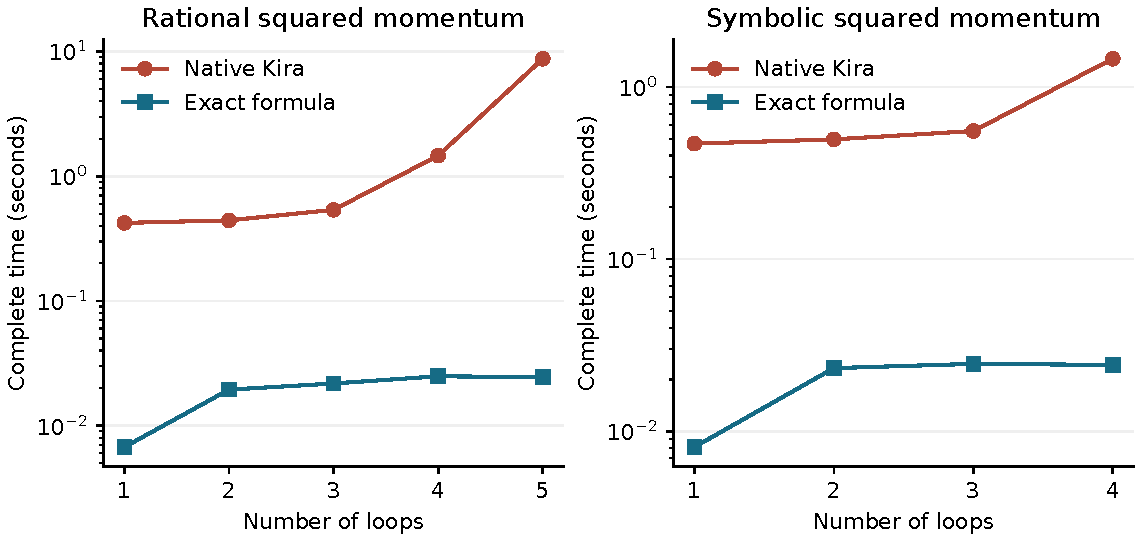
\includegraphics[width=\linewidth]{paper_figures/massless_banana_times.pdf}
\caption{The direct coefficient formula avoids the native equation system for the displayed scalar family. Times include exact coefficient checks. The logarithmic time axis shows both methods, and only completed native comparisons appear. These are analytic gains, separate from ML.}
\label{fig:banana}\end{figure}\FloatBarrier

An additional 240 numerical checks compare the finite rational formula with the uncancelled Gamma-function expression at one through twelve loops and at 16, 24, and 32 loops. They use 70-digit arithmetic at two noninteger dimensions. The general derivation supports this scalar family at every positive loop count; the numerical checks test its implementation at the stated counts. General higher-loop scattering remains outside this analytic specialization.

A separate test starts a new application process for each request. All 48 executions use the combined routing interface, and every successful output passes an exact check. It also passes 49 domain checks. The four analytic requests use one, four, eight, and twelve loops; their summed median application time is 0.6458 seconds. The same formula serves both comparison paths. The 4 matched native requests take 38.161 seconds with the frozen learned workflow and 38.318 seconds with the separately tuned ML-disabled workflow. These native requests repeat the predeclared application subset of the batch study, so they test integration and startup rather than new physical coverage.
